\chapter{Texte}
Innerhalb eines Projekts können Sie beliebig Texte anlegen und verwalten. Hierfür steht Ihnen der \texttt{Projekt Browser} %
zur Verfügung, den Sie im oberen Teil der Navigationsleiste finden (siehe Abbildung \ref{fig:projectbrowser}).

\section{Texte hinzufügen}
\label{sec:newtext}
% 
Um einen neuen Text hinzuzufügen, klicken Sie in der Menüleiste auf \texttt{Project => Create new text} (Abbildung \ref{fig:texthinzu}). %
Alternativ können Sie auch den Mauszeiger über den Project Browser führen und dann die rechte Maustaste klicken.  %

\begin{figure}[!hbt]
\begin{minipage}[!hb!]{0.5\textwidth}
	\centering
	 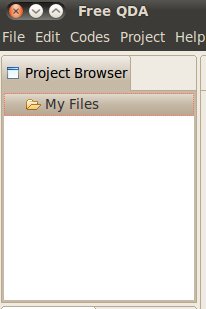
\includegraphics[width=0.5\textwidth]{img/ProjectBrowser}
	\caption{Project Browser}
	\label{fig:projectbrowser}
\end{minipage}
\hfill
\begin{minipage}[!hb!]{0.5\textwidth}
	\centering
	 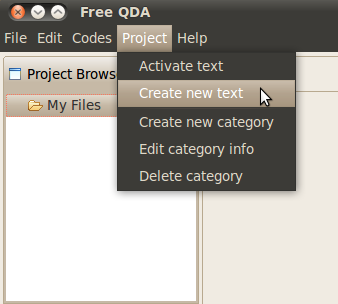
\includegraphics[width=0.8\textwidth]{img/CreateNewText}
	\caption{Text hinzufügen}
	\label{fig:texthinzu}
\end{minipage}
\end{figure}

Es öffnet sich ein neues Fenster, in welchem Sie gebeten werden, den Namen des neuen Textes einzugeben (Abbildung \ref{fig:neuertext1}). %
Geben Sie den Namen ein und klicken Sie \texttt{Finish}. Der neue Text erscheint nun im Project Browser (Abbildung \ref{fig:neuertext2}). 
Durch einen Doppelklick auf den Textnamen öffnen Sie den neuen Text im Editor. Innerhalb des Editors können Sie nun Ihren neuen Text %
schreiben. 
\begin{figure}[!hbt]
\begin{minipage}[!hb!]{0.5\textwidth}
	\centering
	 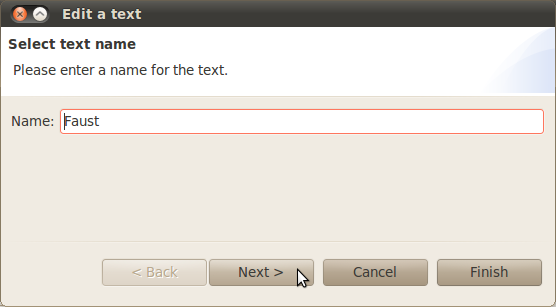
\includegraphics[width=0.8\textwidth]{img/NexText}
	\caption{Textname eingeben}
	\label{fig:neuertext1}
\end{minipage}
\hfill
\begin{minipage}[!hb!]{0.5\textwidth}
	\centering
	 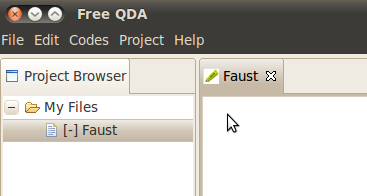
\includegraphics[width=0.8\textwidth]{img/NewText2}
	\caption{Text hinzufügen}
	\label{fig:neuertext2}
\end{minipage}
\end{figure}

Wenn Sie einen Text aus einer bereits bestehenden Datei (z.B. doc, txt, rtf, odt) übernehmen möchten, müssen Sie diese Datei im jeweiligen %
Programm (Word, LibreOffice, etc) öffnen, den gesamten Text dort markieren und in die Zwischenablage kopieren. Jetzt können Sie zum %
FreeQDA-Editor zurückkehren, und den Text mit der Tastenkombination \texttt{STR} und \texttt{V} (bzw. am Mac per  \texttt{APFEL} %
und \texttt{V}) einfügen. 
\begin{figure}[!htb]
	\centering
	 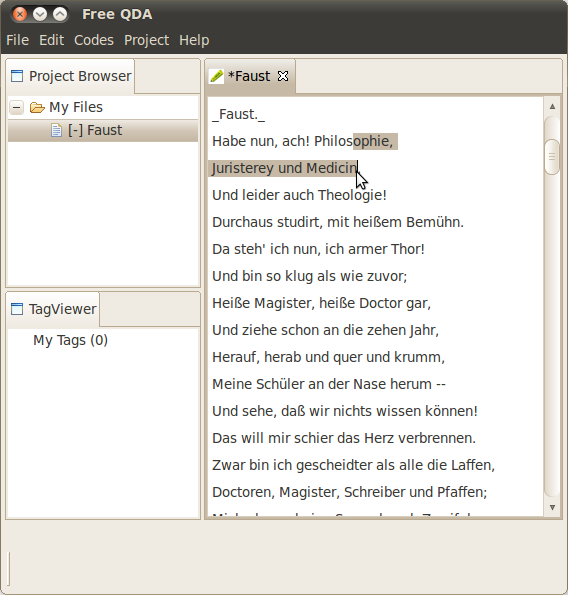
\includegraphics[width=0.4\textwidth]{img/Faust1}
	\caption{Text im Editor}
	\label{fig:faust}
\end{figure}
\vfill

Um den Texteditor zu schließen, klicken Sie in der Tableiste auf das $\times$ Symbol neben dem Textnamen (Abbildung \ref{fig:textschliessen}). %
Das * Symbol vor dem Textnamen (siehe Abbildung \ref{fig:textschliessen} *Faust) bedeutet, dass an dem Text Änderungen vorgenommen wurden, %
die noch nicht gespeichert sind. Wenn Sie den Texteditor schließen, werden Sie daher gefragt, ob Ihre Änderungen gespeichert werden sollen. %
Bestätigen Sie mit \texttt{Yes} um den Text zu speichern. Alle Texte werden übrigens mit der Dateiendung \texttt{fqf} im Projektordner gespeichert (Abbildung \ref{fig:textdatei}). %
Sie sollten diese jedoch nicht mit einem anderen Programm öffnen, da FreeQDA innerhalb der Texte weitere Informationen speichert, welche %
durch andere Programme evtl. überschrieben werden. 
\vfill
\begin{figure}[!hbt]
\begin{minipage}[!hb!]{0.5\textwidth}
	\centering
	 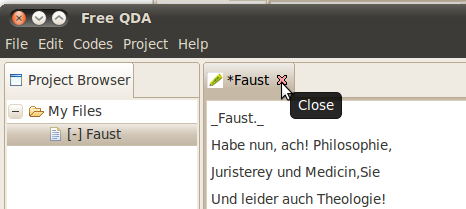
\includegraphics[width=0.8\textwidth]{img/TextSchliessen}
	\caption{Text schließen}
	\label{fig:textschliessen}
\end{minipage}
\hfill
\begin{minipage}[!hb!]{0.5\textwidth}
	\centering
	 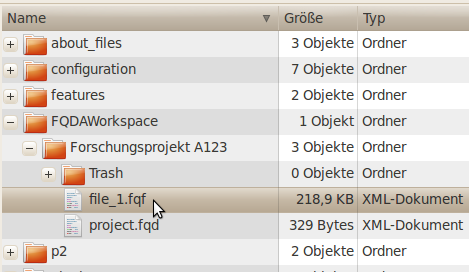
\includegraphics[width=0.7\textwidth]{img/textdatei}
	\caption{Textdatei}
	\label{fig:textdatei}
\end{minipage}
\end{figure}
\newpage
\section{Einen Text löschen}
Um einen Text zu löschen klicken Sie im Project Browser mit der rechten Maustaste auf den gewünschten Text und wählen Sie %
\texttt{Delete Text} (siehe Abbildung \ref{fig:deletetext}).

\begin{figure}[!htb]
	\centering
	 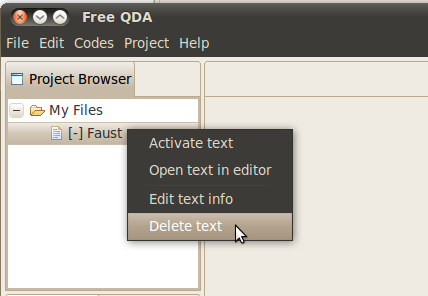
\includegraphics[width=0.4\textwidth]{img/deletetext}
	\caption{Text löschen}
	\label{fig:deletetext}
\end{figure}


\section{Textkategorien}
\label{sec:textcategory}
Texte können in beliebigen Textkategorien verwaltet werden. Um eine neue Textkategorie zu erstellen, klicken Sie in der Menüleiste auf %
\texttt{Project => Create new category} (Abbildung \ref{fig:createnewcategory}). Alternativ können Sie auch innerhalb des Project Browser %
auf die rechte Maustaste klicken. Es öffnet sich ein neues Fenster, in welchem Sie gebeten werden, den Namen der neuen Kategorie %
einzutippen (Abbildung \ref{fig:newcategoryname}). Geben Sie den gewünschten Namen ein und klicken Sie auf \texttt{Finish}. Die neue Kategorie ist nun erstellt.

\begin{figure}[!hbt]
\begin{minipage}[!hb!]{0.42\textwidth}\scriptsize
	\centering
	 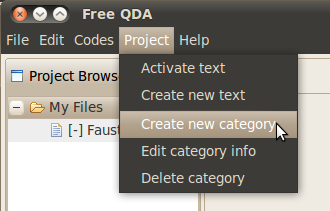
\includegraphics[width=0.7\textwidth]{img/createnewcategory}
	\caption{Textkategorie erstellen}
	\label{fig:createnewcategory}
\end{minipage}
\hfill
\begin{minipage}[!hb!]{0.41\textwidth}
	\centering
	 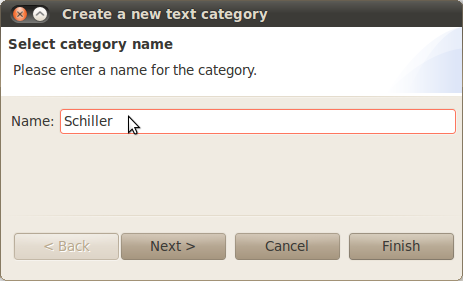
\includegraphics[width=0.75\textwidth]{img/newcategoryname}
	\caption{Kategorie benennen}
	\label{fig:newcategoryname}
\end{minipage}
\hfill
\begin{minipage}[!hb!]{0.15\textwidth}
	\centering \vspace{-26pt}
	 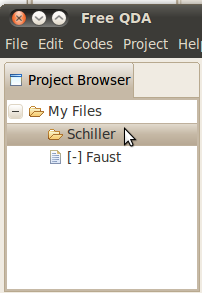
\includegraphics[width=0.9\textwidth]{img/newcategory2}
%	\caption{neue Kategorie}
	\label{fig:newcategory2}
\end{minipage}
\end{figure}


\subsection{Einer Kategorie einen neuen Text hinzufügen}
\begin{wrapfigure}[10]{l}{0.5\textwidth}
 \vspace{-28pt}
 \begin{center}
    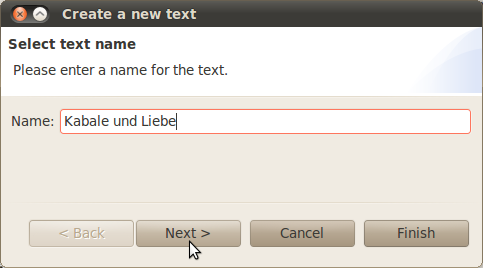
\includegraphics[width=0.45\textwidth]{img/createnewtext3}
  \end{center}
 
	\caption{Klicken Sie auf \texttt{Next}}
	\label{fig:newtext3}
  \vspace{12pt}
\end{wrapfigure}

Um einer Kategorie einen neuen Text hinzuzufügen gehen Sie ähnlich vor wie auf Seite \pageref{sec:newtext}. %  
Klicken Sie im Menü auf \texttt{Project => Create new text}. Es öffnet sich ein neues Fenster, in welchem Sie den Namen des neuen Textes eintragen müssen. %
Klicken Anschließend auf den \texttt{Next} Button (\textbf{nicht} auf den \texttt{Finish} Button, siehe Mauszeiger in Abbildung \ref{fig:newtext3}). Es wird Ihnen nun %
die aktuelle Kategoriestruktur der Texte angezeigt. 
%
\begin{wrapfigure}[12]{l}{0.5\textwidth}
 \vspace{-15pt}
 \begin{center}
    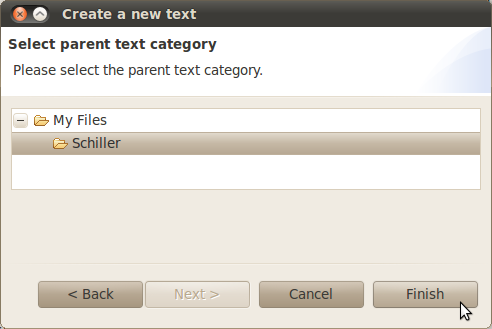
\includegraphics[width=0.45\textwidth]{img/createnewtext4}
	\caption{Kategorie auswählen}
	\label{fig:newtext4}
  \end{center}
  \vspace{12pt}
\end{wrapfigure}
% 
% \begin{figure}[!hbt]
% \begin{minipage}[!hb!]{0.5\textwidth}
% 	\centering
% 	 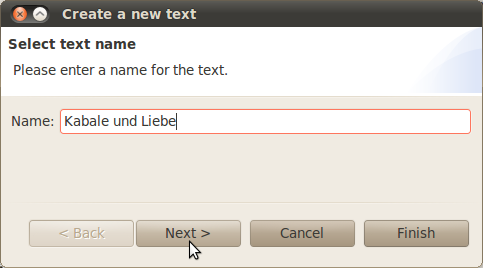
\includegraphics[width=0.8\textwidth]{img/createnewtext3}
% 	\caption{Klicken Sie auf \texttt{Next}}
% 	\label{fig:newtext3}
% \end{minipage}
% \hfill
% \begin{minipage}[!hb!]{0.5\textwidth}
% 	\centering
% 	 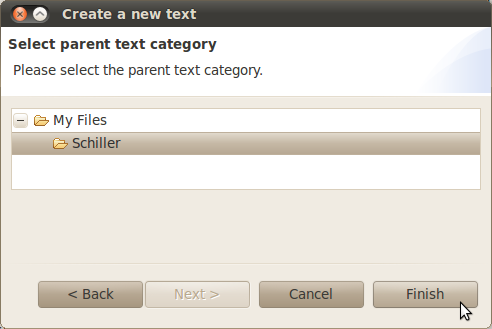
\includegraphics[width=0.7\textwidth]{img/createnewtext4}
% 	\caption{Kategorie auswählen}
% 	\label{fig:newtext4}
% \end{minipage}
% \end{figure}
% 

In unserem Beispiel existiert nur der Ordner \textit{Schiller} (Abbildung \ref{fig:newtext4}). %
Klicken Sie auf den gewünschten Ordner und anschließend auf den \texttt{Finish} Button. 


Die neue Textdatei ist nun im Project Browser unter der genannten Kategorie verfügbar (Abbildung \ref{fig:newtext5}). %
Klicken Sie doppelt auf die Textdatei um den Text im Editor zu öffnen. Innerhalb des Editors können Sie Text %
schreiben oder aus der Zwischenablage einfügen. In Abbildung \ref{fig:newtext5} wurde der Text \textit{Kabale und Liebe} per copy und paste von einer Webseite in den %
Editor übertragen.

Im Project Browser sind alle Kategorien und Texte aufgelistet. Durch Doppelklick auf einen gewünschten Text %
öffnen Sie diesen im Editor. Alle Datein die derzeit im Editor geöffnet sind werden in der Tableiste angezeigt (Abbildung \ref{fig:texttab}). Durch Klicken auf einen %
Tab wechseln Sie zum gewünschten Text. 
\begin{figure}[!hb]
\begin{minipage}[!hb!]{0.5\textwidth}
	\centering
	 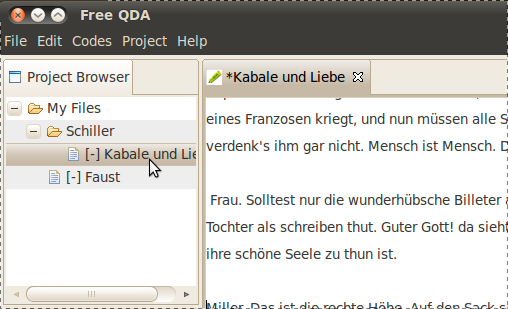
\includegraphics[width=0.75\textwidth]{img/createnewtext5}
	\caption{Textdatei}
	\label{fig:newtext5}
\end{minipage}
\hfill
\begin{minipage}[!hb!]{0.5\textwidth}
	\centering
	 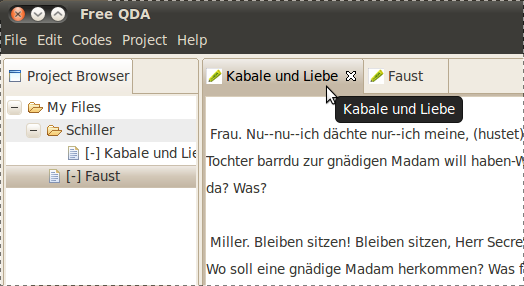
\includegraphics[width=0.8\textwidth]{img/texttab}
	\caption{Texte im Tab}
	\label{fig:texttab}
\end{minipage}
\end{figure}
